%!TEX root = ../main.tex

\chapter{Measure Theory} % (fold)
\label{cha:measure_theory}
\thispagestyle{empty}

\section{Measure spaces} % (fold)
\label{sec:measure_spaces}

Let $X$ be a set.

\begin{defn}[$\sigma$-algebras]$\\$
A family $\Mdu \subset \Peu (x)$ is called a $\sigma$-algebra if 
\begin{enumerate}
    \item[i)] $\emptyset \in \Mdu$
    \item[ii)] $ E \subset \Mdu \ \Longrightarrow \ E^c  = X\setminus E \in \Mdu$
    \item[iii)] $\gr{E_n}_{n \in \mathbb{N}} \subset \Mdu \Longrightarrow \bigcup_{n=1}^{\infty} E_n \in \Mdu $ (infinite countable union)
\end{enumerate}
If (iii) is replaced by "$E_1, E_2 \in \Mdu \Longrightarrow E_1 \bigcup E_2 \in \Mdu$" then $\Mdu$ is just an algebra (finite union).
\end{defn}

Trivial examples: $\Mdu=\Peu(X)$ is the biggest $\sigma$-algebra, $\Mdu=\gr{\varnothing,X}$ is the smallest $\sigma$-algebra.

We say that
\begin{itemize}
    \item $\Mdu$ $\sigma$-algebra $\leadsto$ $(X,\Mdu)$ is a \textbf{measurable space}
    \item $E\in\Mdu$ are \textbf{measurable sets}
\end{itemize}

Basic properties of $\Mdu$:
\begin{enumerate}
    \item $X=\varnothing^c\in\Mdu$ (by (i)+(ii))
    \item $\Mdu$ is an algebra ($\sigma$-alg. $\Longrightarrow$ alg. but not the viceversa)

    To prove this you can take a finite union (e.g. $E_1\cup E_2$) and then make infinite unions with $\varnothing$ to have an infinite union that still belongs to $\Mdu$:
    \begin{equation*}
        E_1\cup E_2=\underbracket[0.5pt]{E_1\cup E_2\underbracket[0.5pt]{\cup\varnothing\cup ... \cup\varnothing\cup...}_{\in\Mdu\text{ by (i)}}}_{\in\Mdu\text{ by (iii)}}
    \end{equation*}

    \item $\gr{E_n}_n\subset\Mdu\Longrightarrow \bigcap_{n\in\NN} E_n\in\Mdu$
    \item $E,F\in\Mdu\Longrightarrow E\setminus F \in \Mdu$
\end{enumerate}

Now, we want to understand how to generate a $\sigma$-algebra.

\begin{thm}$\\$
    Take $\Seu\subset\Peu(X)$ any family. Then it is well defined $\sigma_0(\Seu)$, the $\sigma$-algebra generated by $\Seu$ (the smallest $\sigma$-algebra containing $\Seu$):
    \begin{itemize}
        \item[i)] $\sigma_0(\Seu)$ is a $\sigma$-algebra
        \item[ii)] $\Seu\subset\sigma_0(\Seu)$
        \item[iii)] if $\Mdu$ is a $\sigma$-alg. and $\Seu\subset\Mdu$ then $\sigma_0(\Seu)\subset\Mdu$
    \end{itemize}
\end{thm}

\begin{proof}[Sketch]$\\$
We introduce a collection of collection of sets (we should be more strict: without knowing axiom choices we cannot properly prove this theorem, all we currently need is how to construct these $\sigma$-algebras):
\begin{equation*}
    \Vc=\left\{\Mdu\subset\Peu(X)\,:\,\Mdu\text{ is a }\sigma\text{-alg. and }\Seu\subset\Mdu  \right\}
\end{equation*}
(notice that $\Vc$ is not empty since $\Peu(X)\in\Vc$)

Then $\sigma_0(\Seu)=\bigcap\gr{\Mdu\,:\,\Mdu\in\Vc}$ (to generate the smallest take the intersection of all).
\end{proof}

% section measure_spaces (end)

\section{Borel sets} % (fold)
\label{sec:borel_sets}

We now want to define between measurable and open sets, we do this by constructing the borel $\sigma$-algebra.

\begin{defn}[Borel $\sigma$-algebras and Borel sets]$\\$
    Let $(X,d)$ be a metric space, so that open subsets of $X$ are defined (a topological space is enough) and let $\Teu = \gr{E\subset X\,: \,E \text{ is open}}$. The $\sigma$-algebra generated by $\Teu$, $\sigma_0(\Teu)$, is the Borel $\sigma$-algebra of $X$, and we write $\Bdu (X) = \sigma_0(\Teu)$. 

    Furthermore, any $E\in \Bdu (X)$ is a Borel (measurable) set.
\end{defn}

All the followings are Borel sets:
\begin{itemize}
    \item all open sets
    \item all closed sets (because the $\sigma$-algebra is closed under complements, and the complements of open sets are naturally closed sets)
    \item all countable intersections of open sets (G$\delta$-sets)  
    \item All countable unions of closed sets (F$\sigma$-sets)  
\end{itemize}

We will deal with two main cases:
\begin{itemize}
    \item real numbers $X=\mathbb{R}=(-\infty,+\infty)$
    \item \textit{extended} real numbers $X=\overline{\mathbb{R}} = [-\infty,\infty]$ 
\end{itemize}

\begin{subtle}$\\$
Defining a measure in $\overline{\mathbb{R}}$ isn't trivial, we therefore define how to extend the following operations to $\overline{\mathbb{R}}$.

\textbf{Operations}: let $a\in \mathbb{R}$. Then:
\begin{itemize}
    \item $a>0\ \Longrightarrow\ a\cdot \pm \infty = \pm \infty$
    \item $a<0\ \Longrightarrow\ a\cdot \mp \infty = \pm \infty$
    \item $a\pm \infty = \pm \infty$
    \item $0\cdot \pm \infty = 0$ (note that we are not taking any limits in this assumption, we define it this way because we want the zero function to have a null integral in an unbounded interval)
    \item $+\infty -\infty$ is not defined
\end{itemize}

\textbf{Open intervals}: let $a,b\in\RR$, $a<b$. Then:
\begin{itemize}
    \item $(a,b)$ is open
    \item $[-\infty , b)$ is open
    \item $(a,+\infty ]$ is open
\end{itemize}
\end{subtle}

\newpage

We will deal with $\Bdu(\mathbb{R}) \text{ and }  \Bdu\left(\overline{\mathbb{R}}\right)$.

\begin{marker}
Note that
\begin{align}
        \Bdu(\mathbb{R}) :&= \sigma_0 \left( \gr{\text{open sets}} \right) \nonumber \\
        &=\sigma_0 \left( \gr{\text{open intervals}} \right) \nonumber \\
        &=\sigma_0 \left( \gr{(a,+\infty)}\right) \label{borel_def_3}
\end{align}
This means we can get open sets and open intervals by taking complements, unions and intersections, starting from sets in the form of (\ref{borel_def_3}). This is very useful for proving properties of open intervals and sets. \\
The properties are generally proven more easily when the set of generators is smaller.

Moreover:
    \begin{align*}
        \Bdu(\mathbb{\overline{R}}) :&= \sigma_0 \left( \gr{\text{open sets}} \right) \\
        &=\sigma_0 \left( \gr{(a,+\infty)}\right) \\
        \Bdu(\mathbb{R}^n) :&= \sigma_0 \left( \gr{\text{open rectangles}} \right) \\
        &=\sigma_0 \left( \gr{\text{closed rectangles}} \right)
    \end{align*}
\end{marker}

% section borel_sets (end)

\section{Measures} % (fold)
\label{sec:measures}

Let $(X,\Mdu)$ be a measurable space.

\begin{defn}[Measure]$\\$
A measure on $\Mdu$ is a function 
\begin{equation*}
\mu : \Mdu \longrightarrow [0,+\infty] \quad \text{s.t.} \quad
{\renewcommand*{\arraystretch}{2.5}
\begin{array}{ll}
 \text{i)} & \mu(\varnothing) = 0 \\
 \text{ii)} & \gr{E_n}_n \subset \Mdu \text{ disjoint }\Longrightarrow\ \mu\displaystyle \left( \bigcup_{n\in \NN} E_n \right) = \sum_{n\in \NN} \mu \left( E_n\right)\qquad (\sigma\text{-additivity})
\end{array}}
\end{equation*}
\end{defn}

\begin{defn}[Measure space]$\\$
Take $X,\Mdu,\mu$ as above. Then $ (X,\Mdu,\mu)$ is a measure space.

In particular:
\begin{itemize}
    \item if $\mu(X)=1$ then $ (X,\Mdu,\mu)$ is a probability space and $\mu$ is a probability measure

    \item if $\mu(X)<+\infty$ then $\mu$ is a finite measure

    \item if $\exists \gr{E_n}_n\, :\, \mu \left( E_n \right) < +\infty $ and $ X = \displaystyle\bigcup_n E_n$ then $\mu$ is a $\sigma$-finite measure
\end{itemize}
\end{defn}

Some examples:
\begin{enumerate}
    \item[1)] for any $(X,\Mdu)$\ $\longrightarrow$ \ $\mu \left( E \right) = 0 \ \ \forall E\quad$ is the \emph{trivial measure}

    \item[2)] for any $(X,\Mdu )\  \longrightarrow$ \begin{tabular}[t]{@{}l@{}}
        $\begin{cases}
            \mu(E)=+\infty, &\ \forall E\neq\varnothing \\
            \mu(\varnothing)=0
        \end{cases}\quad$
        \end{tabular} is a measure

    \item[3)] for $(X,\Peu (X) )\  \longrightarrow$ \begin{tabular}[t]{@{}l@{}}
        $\mu_{\#}(E)  =
        \begin{cases}
            \# \gr{\text{elements of } E}, &\text{ if } E\text{ is finite} \\
            +\infty, &\ \text{otherwise}
        \end{cases}\quad$
    \end{tabular} is the \emph{counting measure}
    
    \item[4)] for $(X,\Peu (X) )$ with $X$ nonempty, pick $x_0 \in X \ \longrightarrow$ \begin{tabular}[t]{@{}l@{}}
        $\delta_{x_0}(E)  =$
        $\begin{cases}
            1, &\text{ if } x_0 \in X  \\
            0, & \text{ otherwise}
        \end{cases}\quad$
    \end{tabular} is the \emph{Dirac measure}
\end{enumerate}

% section measures (end)

\newpage

\section{Properties of measure} % (fold)
\label{sec:properties_of_measure}

\begin{thm}[Basic properties]$\\$
Let $(X,\Mdu,\mu)$ be a measure space. Given $E,F\in \Mdu$, we have:
    \begin{itemize}
        \item[i)] Finite additivity: $E\cap F=\varnothing\ \Longrightarrow\ \mu(E\cup F)=\mu(E)+\mu(F)$

        \item[ii)] Excision: $E \subset F$ and $\mu(E)<+\infty \ \Longrightarrow \ \mu(F\setminus E)=\mu(F)-\mu(E)$

        \item[iii)] Monotonicity: $E \subset F\ \Longrightarrow \ \mu(E) \leq \mu(F) $
    \end{itemize}
\end{thm}

\fg{0.5}{SCR20230929}

\begin{proof}\leavevmode
\begin{itemize}
\item[i)] Take $\left\{ E_n \right\}_{n\in\NN}$ s.t.
\begin{equation*}
E_1=E\qquad E_2=F\qquad E_{n\geq 3}=\varnothing
\end{equation*}
Then, thanks to the $\sigma$-additivity we obtain
\begin{equation*}
\mu(E\cup F)=\mu \left( \bigcup_{n\in\NN} E_n \right)=\sum^{\infty}_{n=1} \mu \left( E_n \right)=\mu(E)+\mu(F)+0+\cdots=\mu(E)+\mu(F)
\end{equation*}

\item[ii)] We recall that if $ E,F \in \Mdu \Longrightarrow E \setminus F \in \Mdu $. Then, we notice that $F=E\cup(F\setminus E)$ and the sets $E$ and $(F\setminus E)$ are dsjoint, hence we can apply i):
\begin{equation*}
\mu(F)=\mu\big( E\cup(F\setminus E) \big) = \mu(E)+\mu(F\setminus E)
\end{equation*}

Since $\mu(E)<+\infty$ (to avoid situations where the operation is not defined, e.g. $+\infty-\infty$), we can reverse the equation:
\begin{equation*}
\mu(F\setminus E)=\mu(F)-\mu(E)
\end{equation*}

\item[iii)] Following the same process done in ii):
\begin{equation*}
\mu(F)=\mu(E)+\underbracket[0.2pt]{\mu(F\setminus E)}_{\geq 0}\geq \mu(E)
\end{equation*}
\end{itemize}
\end{proof}

\newpage

\begin{thm}[Continuity along monotone sequences]$\\$
Let $(X,\Mdu,\mu)$ be a measure space and take $\left\{ E_n \right\}_{n\in\NN}\subset\Mdu$.
\begin{enumerate}[(i)]
\item If $\gr{E_n} \nearrow E:= \lim_n E_n = \displaystyle\bigcup_{n=1}^{\infty} E_n $ then      
\begin{equation*}
\mu ( E) = \lim_{n\to\infty} \mu \left( E_n \right)
\end{equation*} 
\item If $\gr{E_n} \searrow E:= \lim_n E_n = \displaystyle\bigcap_{n=1}^{\infty} E_n $ and $\mu \left( E_1 \right)<+\infty$ then
\begin{equation*}
\mu ( E) = \lim_{n\to\infty} \mu \left( E_n \right)
\end{equation*} 
\end{enumerate}
\end{thm}

\begin{proof}[]\leavevmode
\begin{enumerate}[(i)]
\item We define an auxiliary sequence $\left\{ F_n \right\}_n$ s.t. 
\begin{equation*}
F_n=E_n\setminus E_{n-1}\qquad \left( \text{with }E_0:=\varnothing \right)
\end{equation*}
You can check that:
\begin{enumerate}
\item[0)] $F_n\in\Mdu$
\item[1)] $F_i\cap F_j=\varnothing\quad\forall i\neq j$
\item[2)] $\displaystyle E_n=\bigcup_{k=1}^n F_k\quad\Longrightarrow\quad E=\bigcup_{n=1}^\infty F_n$
\end{enumerate}

Now we can freely use the $\sigma$-additivity:
\begin{gather*}
\mu(E)=\mu\left( \bigcup_{n=1}^\infty F_n \right)\overset{\sigma\text{-add.}}{=}\sum^{\infty}_{n=1} \mu\left( F_n \right)=\sum^{\infty}_{n=1} \mu\left( E_n\setminus E_{n-1} \right) =\\
\overset{\text{exc.}}{=}\sum^{\infty}_{n=1} \big[ \mu\left( E_n \right)- \mu\left( E_{n-1} \right) \big] \overset{\text{tel.}}{=}\lim_{n\to\infty}\mu \left( E_n \right)-\underbracket[0.2pt]{\mu \left( E_0 \right)}_{=0}
\end{gather*}

\item We define another disjoint family:
\begin{equation*}
G_n = E_1 \setminus E_n
\end{equation*}

Check that:
\begin{enumerate}
\item[0)] $G_n \in \Mdu$
\item[1)] $\gr{G_n} \nearrow$
\item[2)] $\displaystyle\bigcup_{n=1}^{\infty} G_n = E_1 \setminus \bigcap_{n=1}^{\infty} E_n = E_1 \setminus E$
\end{enumerate}

On one hand
\begin{equation*}
\mu\left( \bigcup_{n=1}^{\infty} G_n \right) \overset{(\text{i})}{=} \lim_n \mu\left( G_n \right) \overset{\text{exc.}}{=} \lim_n \big[ \mu\left( E_1 \right)- \mu\left( E_{n}\right) \big] = \mu\left( E_1 \right)-\lim_n \mu\left( E_{n} \right)
\end{equation*}
but on the other hand
\begin{equation*}
\mu\left( \bigcup_{n=1}^{\infty} G_n \right) \overset{2)}{=} \mu\left( E_1 \right)-\mu(E)
\end{equation*}

Since $\mu\left( E_1 \right)<+\infty$ we can simplify the terms and finally obtain $\mu ( E) = \displaystyle\lim_{n\to\infty} \mu \left( E_n \right)$.
\end{enumerate}
\end{proof}

\begin{subtle}$\\$
In (ii) the assumption $\mu\left( E_1 \right)<+\infty$ is essential (it cannot be removed). If you don't believe it, consider $\left( \NN,\Peu\left( \NN \right),\mu_{\#} \right)$ and $E_n=\left\{ k\in\NN\,:\,k\geq n \right\}$:
\begin{equation*}
{\renewcommand*{\arraystretch}{1.1}
\begin{array}{ccccc}
E_{n+1}\subset E_n &\Longrightarrow &\mu_{\#}\left( E_n \right)=+\infty\quad\forall n &\Longrightarrow &\lim_n\mu_{\#}\left( E_n \right)=+\infty \\
&&&&\neq \\
\forall m\in\NN,\ m\notin E_{m+1}&\Longrightarrow &E=\lim_n E_n=\displaystyle\bigcap_n E_n=\varnothing&\Longrightarrow &\mu_{\#}(E)=0
\end{array}}
\end{equation*}
\end{subtle}

\begin{thm}[$\sigma$-subadditivity]$\\$
Let $(X,\Mdu,\mu)$ be a measure space and take $\left\{ E_n \right\}_{n\in\NN}\subset\Mdu$. Then:
    \begin{equation*}
        \mu \left( \bigcup_{n=1}^{\infty} E_n \right) \leq \sum_{n=1}^{\infty} \mu \left( E_n \right)
    \end{equation*}
\end{thm}

So, weakening the hypothesis of disjoint sets we lose the = and we get the $\leq$.

\begin{proof}$\\$
We define an auxiliary sequence of sets:
\begin{equation*}
\left\{
{\renewcommand*{\arraystretch}{2.5}
\begin{array}{ll}
F_1 = E_1 & \\
F_n = E_n \setminus \left( \displaystyle\bigcup_{k=1}^{n-1} E_k \right) & \forall n \geq 2
\end{array}}
\right.
\end{equation*}

These are measurable, disjoint and
\begin{equation*}
\bigcup_{n=1}^{\infty}  F_n  = \bigcup_{n=1}^{\infty} E_n 
\end{equation*}
(so we can use $\sigma$-aditivity)

Therefore:
\begin{equation*}
\mu \left( \bigcup_{n=1}^{\infty} E_n \right) = \mu \left( \bigcup_{n=1}^{\infty} F_n \right)
\overset{\underset{\sigma\text{-add.}}{}}{=} \sum_{n=1}^{\infty} \mu \left( E_n \right)
\overset{\underset{\Rightarrow \text{ monot.}}{\scriptscriptstyle{F_n\subset E_n\forall n}}}{\leq}
\sum_{n=1}^{\infty} \mu \left( E_n \right)
\end{equation*}
\end{proof}


\begin{marker}[]$\\$
If $f: \Mdu to \left[ 0, +\infty \right]$ is finitely-additive and $\sigma$-subadditive then $f$ is also $\sigma$-additive. We'll seldom use this fact , but it is important to know that these are all linked properties. 

In addition, this is the most practical way to confirm that something is a measure:
\begin{equation*}
\mu(\varnothing)=0\qquad + \qquad \text{finite additivity} \qquad+\qquad\sigma\text{-subadditivity}
\end{equation*}
\end{marker}

% section properties_of_measure (end)

\newpage

\section{Negligible sets (sets of zero measure)} % (fold)
\label{sec:negligible_sets_}

Let $(X,\Mdu,\mu)$ be our measure space.

\begin{defn}[Negligible sets]\leavevmode
    \begin{itemize}
        \item N $\in \Mdu$ has zero measure if $\mu (N) = 0$
        \item F $\subset X$ is negligible (\emph{trascurabile}) if $F \subset N$ where $N$ has zero measure
    \end{itemize}
\end{defn}

\begin{subtle}$\\$
Negligible sets are not generally measurable, but they have zero measure when they are:
\begin{equation*}
{\renewcommand*{\arraystretch}{1.5}
\begin{array}{lllll}
&&F\notin\Mdu&\Longrightarrow&\mu(F)\text{ not defined} \\
&\nearrow&&& \\
F\subset X&&&& \\
&\searrow&&& \\
&&F\in\Mdu&\Longrightarrow&\mu(F)\text{ well defined, and for monotonicity:} \\
&&&&\qquad\mu(F)\overset{\scriptscriptstyle{F\subset N}}{\leq}\mu(N)=0\Rightarrow\mu(F)=0
\end{array}}
\end{equation*}
\end{subtle}

\begin{defn}[Complete measures and Complete measure spaces]$\\$
$\mu$ is complete $\big($or $(X,\Mdu,\mu)$ is complete$\big)$ if every negligible set belongs to $\Mdu$.
\end{defn}

A measure space $(X,\Mdu,\mu)$ needs not to be complete. However, by defininig
\begin{equation*}
    \overline{\Mdu} := \gr{E \subset X \,:\, \exists F_1,F_2 \in \Mdu \text{ s.t. } F_1 \subset E \subset F_2\text{ and }\underbracket[0.2pt]{\mu \left( F_2 \setminus F_1 \right) = 0}_{\text{or }\mu\left( F_1 \right)=\mu\left( F_2 \right)}}_{\qquad (\text{"trap E"})}
\end{equation*}

\begin{figure}[H]
\begin{center}
  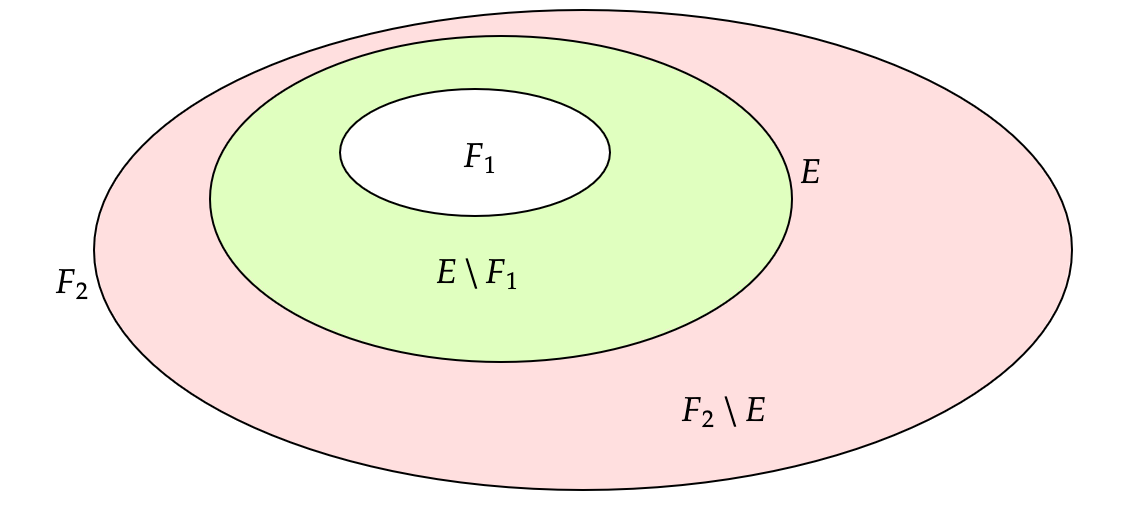
\includegraphics[width=8cm]{SCR-20231001-kkwz}
\end{center}
\caption*{Note that both $E\setminus F_1$ and $F_2\setminus E$ are $\subset F_2\setminus F_1$ $\Longrightarrow$ they're both negligible.}
\end{figure}

you get a $\sigma$-algebra. Moreover, for every set $E \in \overline{\Mdu}$ and $F_1,F_2$ by defininig
\begin{equation*}
    \overline{\mu} \left( E \right) := \mu \left( F_1 \right) = \mu \left( F_2 \right)
\end{equation*}
you get a complete measure on $\overline{\Mdu}$. And so yopu have created a new measure space, $\left( X,\overline{\Mdu},\overline{\mu} \right)$, which is complete (we do not prove this fact, but we'll use it).

% section negligible_sets_ (end)

% chapter measure_theory (end)




